Priponsko drevo nad besedo $T$ dolžine $n$ potrebuje za vsako vozlišče vsaj en kazalec ter dva \enquote{cela števila}, ki predstavljata začetek in konec predstavljenega podniza, zato se potrebuje vsaj $6n$ \enquote{celih števil} (bolj natančno $6n\log{n}$ bitov). Pri tem se potrebuje še $n$ dodatnih \enquote{celih števil} za shraniti priponske povezave, dodatnih $2n$ \enquote{celih števil} za shraniti povezave na starše vozlišč ter še dodatnih $n$ \enquote{celih števil} za shraniti indekse pripon, ki so shranjeni v listih. Torej priponsko drevo potrebuje med $7n$ in $10n$ \enquote{celih števil} za pravilno delovanje. Ker so pripone besedila indeksi v besedilu, ki predstavljajo indeks prvega znaka v priponi, se jih lahko shrani z $n$ \enquote{celimi števili}. Če se indekse pripon shranjenih v polju in se indeksi uredijo v leksikografskem vrstnem redu pripon, se ta podatkovna struktura imenuje priponsko polje (angl. \textit{Suffix array} oziroma SA).

\begin{figure}[htb]
    \begin{subfigure}[t]{\linewidth}
        
        \includesvg{Slike/KOKOŠMcCreightS1.svg}
        \centering
        \subcaption*{}
        \label{fig:aSADrevo}
    \end{subfigure}
    \begin{subfigure}[t]{1\linewidth}        
        \includesvg[scale=1.2]{Slike/KokosSA.svg}
        \centering
        \subcaption*{}
        \label{fig:aSAPolje}
    \end{subfigure}
    \caption{Primer priponskega polja nad besedo \enquote{KOKOŠ$\$$}.} 
    \label{fig:SuffuxArray}
\end{figure}

Priponsko polje je alternativni indeks besedila. Priponsko polje se uporablja namesto priponskega drevesa, ko se potrebuje prostorsko bolj učinkovito podatkovno strukturo in se lahko žrtvuje čas iskanja vzorcev v besedilu saj priponsko polje zasede približno 8-krat manj prostora na delovnem pomnilniku kot priponsko drevo \cite{Manber1990}. Priponsko polje si lahko predstavljamo kot polje listov priponskega drevesa, brez podatkov o notranjih vozliščih drevesa. To podobnost lahko vidimo tudi na Sliki \ref{fig:SuffuxArray}, na kateri je prikazano priponsko drevo in priponsko polje za besedo \enquote{KOKOŠ$\$$}.

V nadaljevanju poglavja bodo predstavljena še podatkovna struktura, ki omogoča hitrejše iskanje v priponskem polju ter simuliranje priponskega drevesa. Zatem bodo predstavljeni še načini izgradnje priponskega polja ter implementacije poizvedb s pomočjo priponskega polja.

%\begin{figure}[htb]
%    \begin{center}
%        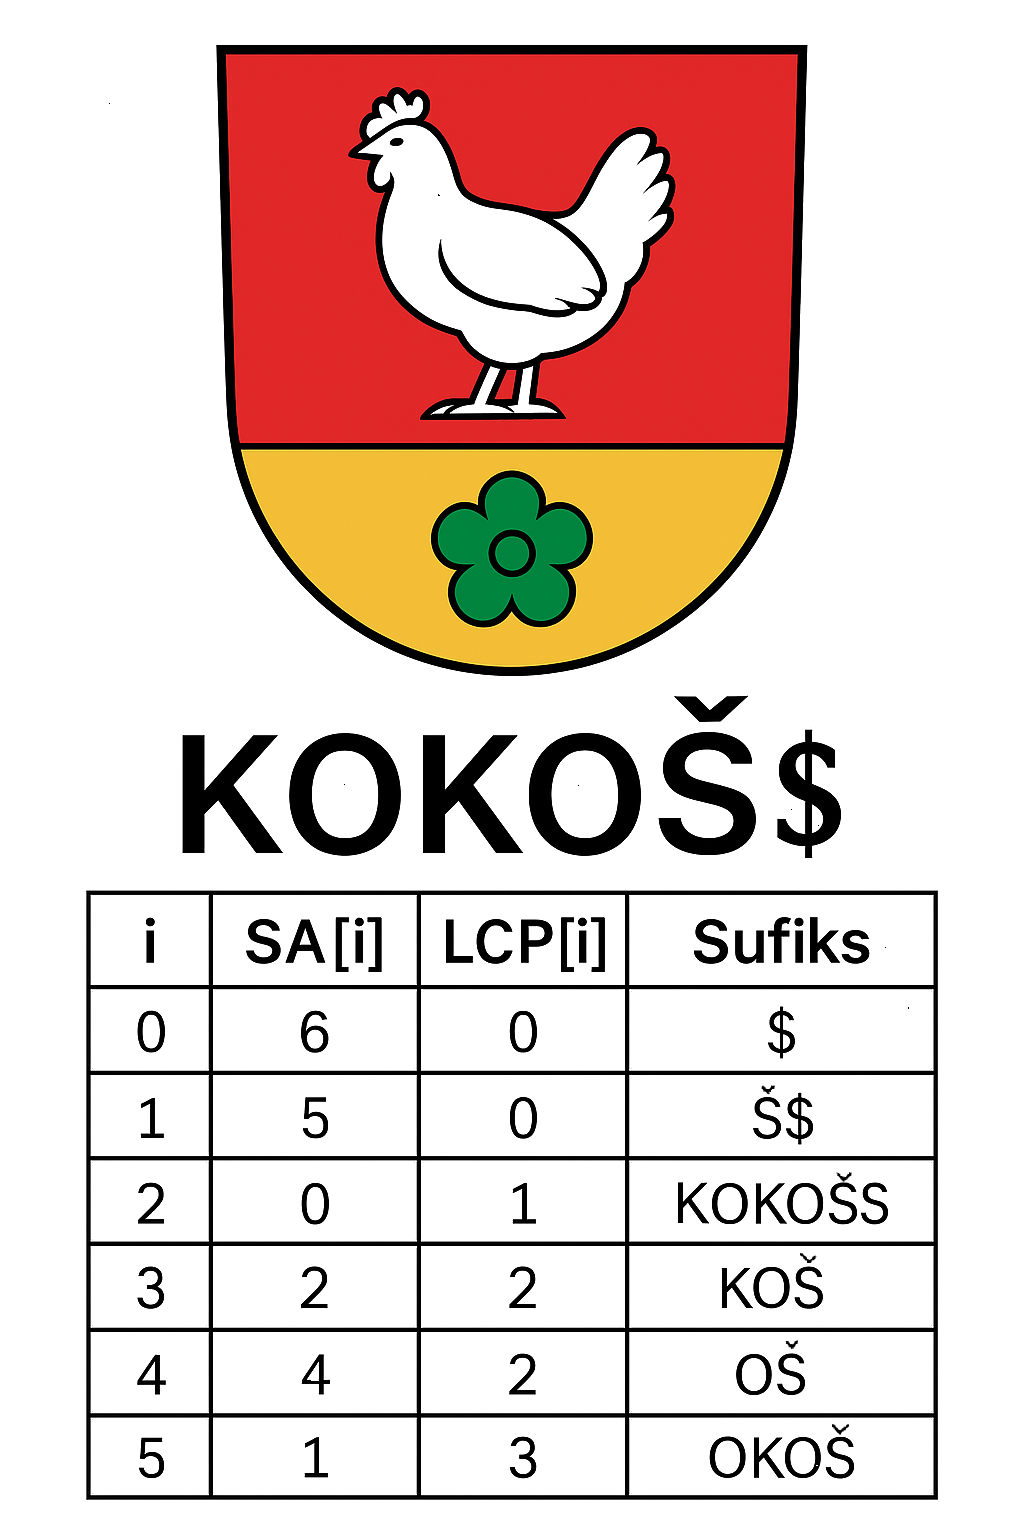
\includegraphics[width=.5\textwidth]{Slike/ChatGPTSA.png}
%        \caption{Primer priponskega polja nad besedo \enquote{KOKOŠ$\$$} kot si jo predstavlja ChatGPT.} 
%        \label{fig:ChatGPT}
%    \end{center}
%\end{figure}



\section{SKUPNA NAJDALJŠA PREDPONA}\label{sec:LCP}
\import{.}{PriponskoPolje/LCP}

\newpage

\section{IZGRADNJA}\label{sec:SAIzgradnja}
\import{.}{PriponskoPolje/Izgradnja}

\newpage

\section{POIZVEDBE}\label{sec:SAPoizvedbe}
\import{.}{PriponskoPolje/Poizvedba}